\chapter{Introduction}
% Approximately 1000 words

% Address why cycling is to be encouraged
The world is engulfed in the midst of a climate emergency and Ireland has among the highest per capita emissions in the European Union. In 2022, Ireland emitted 13.09 kt of CO\textsubscript{2} equivalent greenhouse gasses per person; the third highest in the EU \citep{eeaEEAGreenhouseGases2024}. Of this, transportation represents 19.1\% and while the CO\textsubscript{2} intensity of private car use has been steadily decreasing, it consistently represents some 40\% of total transportation emissions \citep{walshEnergyIreland20202021}. Research into Ireland's transport habits undertaken in \citet{ntaNationalHouseholdTravel2022}, has discovered that a majority of trips (63\%) taken in Dublin city and suburbs and close to half of national trips (49\%) are less than 5km in length. In the face of this existential emergency these journeys can and should be done by sustainable modes where possible. In fact the modal share of journeys in this length range has been effectively entirely occupied by sustainable modes in countries which actively encourage them such as the Netherlands \citep{tonCyclingWalkingDeterminants2019}.

\begin{figure}[hbt!]
    \centering
    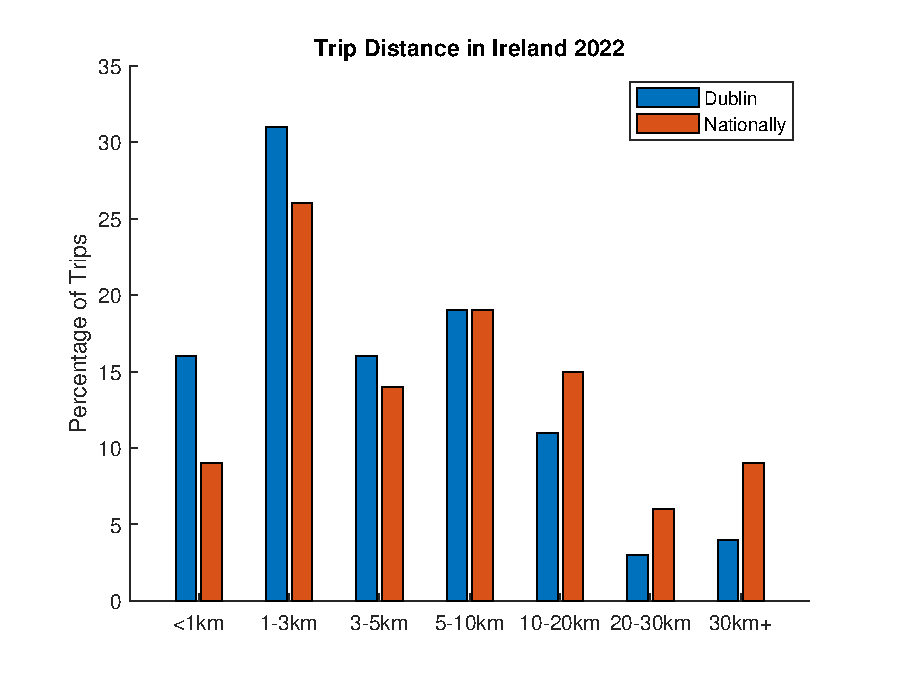
\includegraphics[width=0.60\linewidth]{figures/Irish_trip_distance.eps}
    \caption{Proportion of Trip Distances Nationally and in Dublin \citep{ntaNationalHouseholdTravel2022}}
    \label{fig:TripDistances}
\end{figure}

One of these sustainable modes, and the focus of this thesis is cycling. Cycling has clear and well understood benefits to the environment, health, business, governmental infrastructural spending and synergies with other sustainable transport modes \citep{fraserCyclingTransportPublic2011,kagerCharacterisationReflectionsSynergy2016, dehartogHealthBenefitsCycling2010}. A pivotal study describing a robust cost-benefit analysis used in Copenhagen concluded that per kilometer, cycling has a cost to society less than a sixth that of motoring \citep{gosslingTransportTransitionsCopenhagen2015}. Due to these factors cycling is well regarded as a critical piece of the sustainable network of interventions that will be required to address the climate crisis and de-carbonise transportation.

% Address that we are pushing for better/effective infrastructure
As a result of these clear benefits governmental policy has shifted in recent years to have a greater emphasis on driving a modal shift to cycling from private car use where feasible. However, a frequently citied barrier to this modal shift is danger; both perceived and actual \citep{lawsonPerceptionSafetyCyclists2013}. While it is well understood that the most effective measures to reduce both fatalities and casualties is the introduction of segregated cycling infrastructure. There has been an under-delivery relative to Government targets \citep{ginty2023YearReview2023}. In conjunction with this there has been widespread criticism that the current approach of the Road Safety Authority (RSA) has been sorely lacking in the promotion and facilitation of this most effective intervention. Instead, the RSA has repeatedly focused their efforts on a number of awareness campaigns to try influence both driver and cyclist behaviour \citep{nugentCyclistsPedestriansAre2015, mcgreevyRoadCyclistsWe2024, rsaCyclistsCampaignRoad2022}. The effectiveness of these public information campaigns is difficult, if not impossible to quantify as there is no empirical measure of their impact on driver behaviour. It is vital that future campaigns rely on evidence-based practices and understanding of the decision making mechanisms behind behaviour. This project may be a step in providing the required framework for that change.

However, in the absence of fully segregated infrastructure, situations exist where interaction between cyclist and motorists is inevitable. Therefore, there is merit in examining the factors that influence driver perception and decision making during these interactions. An interaction of particular note which is commonly observed is a compulsive unsafe overtaking behaviour of cyclists where no benefit is imparted onto the driver. Examples of these situations are when approaching a junction or a red light. This is a fascinating scenario, why would someone choose to make a more dangerous decision for no gain? What are the basic underlying mechanisms behind the poor evaluation of these situations?

% What is the current situation of how we deal with cyclists in a road safety environment
The statistics regarding these interactions are alarming. Vulnerable road users (VRUs), those users who are not protected by the bodywork of a vehicle, are not a majority of those using Irish roads; in 2019 they represented some 15\% of annual journeys on the road network and a significantly smaller proportion of kilometers travelled \citep{constantProtectingVulnerableRoad2010, departmentoftransportTransportTrends20202020}. However, they are disproportionally represented in Irish crash statistics with 25\% of fatalities in the same year being VRUs \citep{rsaProvisionalReviewFatal2021}. This headline fatality figure also fails to represent the hundreds of injuries that do not get reported to An Garda Síochána (AGS). A recent publication by the RSA details that "the number of injured child cyclists recorded in Irish hospital data is more than six times higher than in records kept by AGS" and that the overall number of cyclists hospitalised was nearly 2.5 times the figures reported by the Gardaí \citep{castelloSeriousInjuriesPedal2023}.

% Why can this framework of decision neuroscience be used to determine the
In order to examine what governs the decision making process during the driver/cyclist interaction, this thesis will endeavour to study the underlying behaviour using the tools of decision neuroscience (DN). The study of human decision making has a wide rooted history in many disciplines from early philosophical inquires to studies of 'bounded rationality' in the mid 20th century with the area now known as behavioural economics emerging in the 1970s \citep{jonesBOUNDEDRATIONALITY1999,kaoBehaviouralEconomicsClassical2015}. Humans make complicated and difficult to appraise decisions at an incredible rate, influencing every aspect of our lives. It is of no surprise therefore, that it has been studied from so many perspectives due to its vast implications on human behaviour. In recent years, from its roots in psychology, philosophy and economics, a field evolved with a far greater focus on the neural mechanisms behind decisions. It is this field which is the foundation of this project.

Decision neuroscience (DN) is the application of neuroscience to the study of human decision making. It aims to not only understand the decision, but also the process through which the brain makes that decision. This takes the form of creating models to characterise the various mechanisms involved in making a decision \citep{ratcliffDiffusionDecisionModel2008}. It's mechanistic based approach revolutionised the field of decision studies, becoming a standard method of research in the area.

Driver psychology and decision-making has been studied in the past as a method of determining, quantifying and reducing the risks associated with driving. More concretely for the subject of this thesis, research has been conducted within the DN field with regard to road safety \citep{pekkanenVariableDriftDiffusionModels2022}. However, a gap in the literature exists where driver decisions have not been characterised with regard to VRUs.

It is the aim of this thesis therefore, to examine the decisions made by drivers with regard to cyclists, to quantify their biases and to investigate the factors which influence risky behaviour on the roads. This was conducted through the creation of a minimally realistic task, capable of capturing the required behavioural data to allow for the extrapolation of the fundamental cognitive factors at play during risky driving behaviour. The task was designed in such a manner that its results could be fit to the mechanistic models that give DN its power. However, the task construction, piloting and validation ended up requiring the bulk of the technical work during the project timeline so this modelling will have to be conducted as future work.